\documentclass[conference, 12pt]{IEEEtran}
\usepackage{graphicx}
\usepackage{amsmath}
\usepackage{multirow}
\usepackage{hyperref}
\usepackage{float}

\title{Graph Data Science for Author Domain Classification and Link Prediction}

\author{\IEEEauthorblockN{Basil Ali Khan, Hamza Ansari, Hayyan Khan} \\
\IEEEauthorblockA{Group 6\\ Graph Data Science, Spring 2025}}
\pagestyle{plain}
\begin{document}

\maketitle

\section{Introduction}
The source code used in this project is available on GitHub at the following link: 
\href{https://github.com/basil-ali-khan/Node_Classification_and_Link_Prediction_Using_Neo4j}{GitHub Repository}.

\section{Data Cleaning and Preprocessing}
The raw dataset, sourced from \cite{10.1162/qss_a_00163}, comprised several CSV files: \texttt{authors.csv}, \texttt{journal.csv}, \texttt{paper.csv}, \texttt{topic.csv}, \texttt{paper\_journal.csv}, \texttt{paper\_topic.csv}, and \texttt{paper\_reference.csv}. To ensure data quality and consistency, we performed extensive cleaning and preprocessing using R scripts.

For \texttt{paper.csv}, missing values in \texttt{paper\_citation\_count} were imputed with 0, and rows lacking essential fields such as \texttt{paper\_id}, \texttt{paper\_year}, or \texttt{journal\_date} were removed. In \texttt{journal.csv}, missing \texttt{journal\_publisher} entries were set to ``Unknown'', and duplicates in \texttt{journal\_name} were consolidated by merging publisher information. Fuzzy matching was employed to standardize publisher names, addressing variations like ``Routledge'' and ``Routledge Journals''. This method didn't turn out to be very fruitful so we ended up standardizing using the first significant names of publishers to ensure consistency across \texttt{paper\_journal.csv}.

For \texttt{topic.csv}, duplicates based on \texttt{topic\_id} and \texttt{topic\_name} were eliminated, and topic names were standardized to title case. In relationship files (\texttt{paper\_reference.csv}, \texttt{paper\_topic.csv}, \texttt{paper\_journal.csv}), entries with invalid references (e.g., IDs not present in corresponding node files) were discarded to maintain referential integrity. The R scripts for data cleaning are available in the GitHub repository under \texttt{gdscleaning.R} and \texttt{gdscleaning2.R}.

Post-cleaning, the dataset was refined, ensuring only high-quality data was utilized for graph construction in Neo4j. The number of rows before and after cleaning for each file is summarized in Table \ref{tab:cleaning_stats}. 

\begin{table}[h]
\centering
\caption{Row Counts Before and After Data Cleaning}
\label{tab:cleaning_stats}
\begin{tabular}{|l|c|c|}
\hline
\textbf{File} & \textbf{Rows Before} & \textbf{Rows After} \\
\hline
\texttt{authors.csv} & [38926] & [38926] \\
\texttt{author\_paper.csv} & [56541] & [56541] \\
\texttt{journal.csv} & [166] & [166] \\
\texttt{paper.csv} & [693753] & [69362] \\
\texttt{topic.csv} & [6490] & [6471] \\
\texttt{paper\_journal.csv} & [32648] & [32648] \\
\texttt{paper\_topic.csv} & [41881] & [41723] \\
\texttt{paper\_reference.csv} & [1132045] & [1048576] \\
\hline
\end{tabular}
\end{table}

\section{Graph Construction}
Using the cleaned dataset, we constructed a heterogeneous graph in Neo4j to represent relationships between authors, papers, topics, journals, and publishers in the academic domain. The graph model was designed to facilitate both node classification and link prediction tasks.

\subsection{Nodes}
\begin{itemize}
    \item \textbf{Author}: Represents researchers. Properties include:
    \begin{itemize}
        \item \texttt{id}: Unique identifier.
        \item \texttt{name}: Author name.
        \item \texttt{total\_citations}: Sum of citations for authored papers.
        \item \texttt{research\_domain}: Most frequent research topic.
        \item \texttt{last\_collab\_year}: Most recent collaboration year.
    \end{itemize}
    \item \textbf{Paper}: Represents academic papers. Properties include:
    \begin{itemize}
        \item \texttt{id}: Unique identifier.
        \item \texttt{title}: Paper title.
        \item \texttt{year}: Publication year.
        \item \texttt{citationCount}: Citation count.
    \end{itemize}
    \item \textbf{Topic}: Represents research topics. Properties include:
    \begin{itemize}
        \item \texttt{id}: Unique identifier.
        \item \texttt{name}: Topic name.
    \end{itemize}
    \item \textbf{Journal}: Represents journals. Properties include:
    \begin{itemize}
        \item \texttt{name}: Journal name.
    \end{itemize}
    \item \textbf{Publisher}: Represents journal publishers. Properties include:
    \begin{itemize}
        \item \texttt{name}: Publisher name.
    \end{itemize}
\end{itemize}

\subsection{Relationships}
\begin{itemize}
    \item \textbf{WROTE}: Connects \texttt{Author} to \texttt{Paper}.
    \item \textbf{CO\_AUTHORED}: Connects two \texttt{Author} nodes who collaborated. Includes:
    \begin{itemize}
        \item \texttt{collaboration\_year}: Year of collaboration.
    \end{itemize}
    \item \textbf{HAS\_TOPIC}: Connects \texttt{Paper} to \texttt{Topic}.
    
    \item \textbf{PUBLISHED\_IN}: Connects \texttt{Paper} to \texttt{Journal}.
    \item \textbf{PUBLISHED\_BY}: Connects \texttt{Journal} to \texttt{Publisher}.
    \item \textbf{CITES}: Connects \texttt{Paper} to another cited paper.
\end{itemize}

\begin{figure}[h]
    \centering
    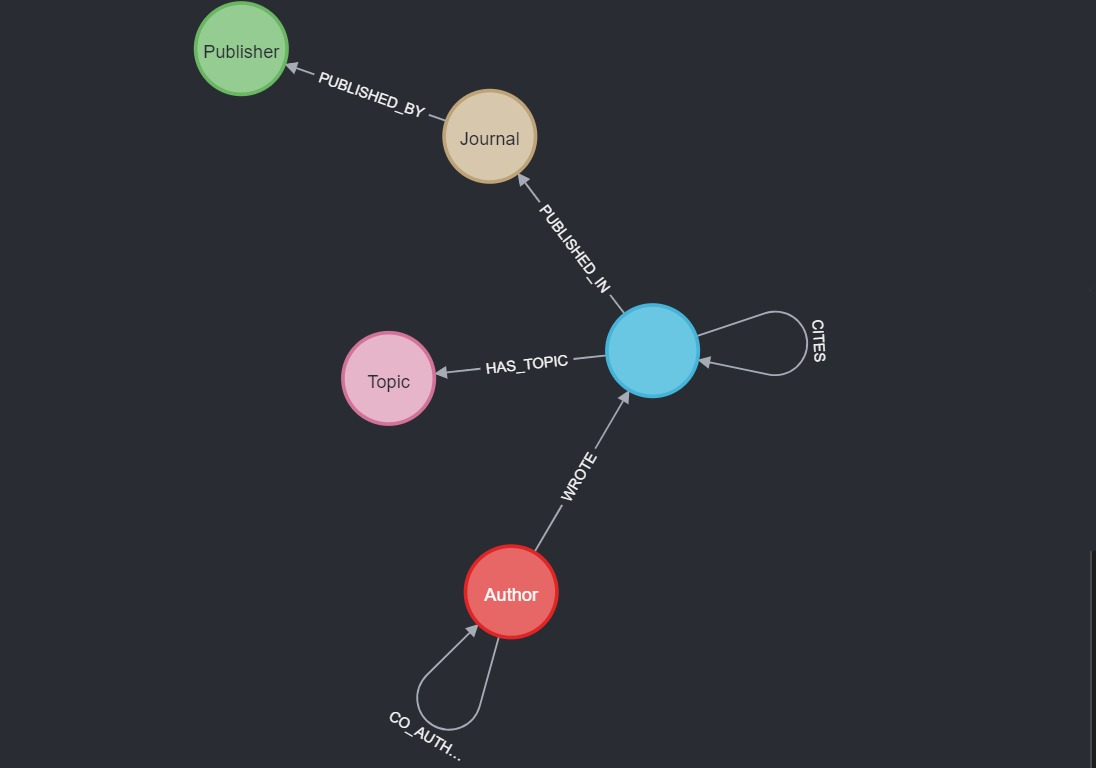
\includegraphics[width=\linewidth]{graph_model.jpg} 
    \caption{Data Model for the Graph}
    \label{fig:data_model}
\end{figure}

\subsection{Feature Engineering}
Additional features were computed to enhance the graph model:
\begin{itemize}
    \item \textbf{Total Citations}: Sum of citations for an author's papers.
    \item \textbf{Research Domain}: Most frequent topic researched by an author.
    \item \textbf{Last Collaboration Year}: Most recent year of collaboration.
\end{itemize}

\subsection{Neo4j Script for Graph Creation}
The Neo4j script for graph construction is available in the GitHub repository under \texttt{graph\_model\_creation\_script.txt}.

\section{Methodology}

\subsection{Node Classification}
The node classification task aimed to predict the research domain (\texttt{domain\_id}) of authors based on their co-authorship patterns and other features. We utilized the Neo4j Graph Data Science (GDS) library to train a machine learning model to classify authors into specific research domains. The authors were represented as nodes in a co-authorship graph, where edges between nodes (authors) represented collaborations (co-authorships) in academic papers.

\subsubsection{Graph Projection}
The first step in our methodology was to project the graph as follows:
\begin{itemize}
  \item \textbf{Nodes:} 
    \begin{itemize}
      \item \texttt{Author}: Represents an academic author. Each author node has a property \texttt{domain\_id} (the target classification label).
    \end{itemize}
  \item \textbf{Relationships:} 
    \begin{itemize}
      \item \texttt{CO\_AUTHOR}: Represents a collaboration between two authors on a paper.
    \end{itemize}
  \item \textbf{Label:} Authors with known research domains were tagged with the label \texttt{AuthorWithDomain} for the classification task. Authors without a known \texttt{domain\_id} were excluded, leaving 12,738 authors (approximately 32.7\% of the total 38,925).
\end{itemize}

\subsubsection{Feature Engineering}
To predict the \texttt{domain\_id}, we used the following features:
\begin{itemize}
  \item \textbf{Louvain Community ID}: Generated using the Louvain algorithm to detect communities based on co-authorship patterns, useful for domain classification.
  \item \textbf{Graph Embedding}: Generated using Fast Random Projection (FastRP) to transform the graph structure into a vector space, capturing local and global network structure. Embeddings of dimensions 64 and 128 were tested.
  \item \textbf{Domain ID}: The target property for classification.
\end{itemize}

\subsubsection{Machine Learning Model}
We used a Random Forest classifier, chosen for its robustness to overfitting and effectiveness with high-dimensional data. The training process included:
\begin{itemize}
  \item \textbf{Random Forest Classifier}: Configured with 25 or 40 trees in different iterations.
  \item \textbf{5-Fold Cross-Validation}: To ensure generalization.
  \item \textbf{Evaluation Metrics}: F1-Weighted, Accuracy, Out-of-Bag (OOB) Error.
\end{itemize}

\subsubsection{Model Training and Evaluation}
The model was trained using a pipeline that included feature extraction (Louvain, FastRP), model training, and cross-validation. Predictions were made on unseen nodes to assess performance.

\subsection{Link Prediction}
The link prediction task aimed to forecast future collaborations between authors based on their historical co-authorship patterns and associated features. We leveraged the Neo4j GDS library's link prediction pipeline, integrating graph algorithms and machine learning to predict potential links.

\subsubsection{Graph Projection}
We projected a graph with:
\begin{itemize}
  \item \textbf{Nodes}: \texttt{Author} nodes with properties \texttt{paper\_count} and \texttt{citation\_count}.
  \item \textbf{Relationships}: \texttt{CO\_AUTHORED} relationships, representing past collaborations, treated as undirected.
\end{itemize}

\subsubsection{Feature Engineering}
To capture graph structure, we experimented with embedding techniques:
\begin{itemize}
  \item \textbf{Initial Approach}: A heuristic-based method was developed to compute similarity scores for author pairs. This involved identifying influential authors using PageRank, selecting potential collaborators based on domain and publication criteria, and calculating scores based on normalized paper and citation counts, domain similarity, and citation relationships. This approach provided a baseline for comparison with machine learning models. This score was not used in the final model but could serve as a feature in future pipelines.
  \item \textbf{FastRP Embeddings}: Used in the second iteration to generate 64-dimensional embeddings efficiently.
  \item \textbf{Node2Vec Embeddings}: Used in the final model, generating 64-dimensional embeddings via biased random walks (walk length 80, 10 walks per node) to capture local and global structures.
\end{itemize}
Features were extracted using the Hadamard product of node embeddings.

\subsubsection{Machine Learning Model}
We trained a logistic regression model to classify potential links:
\begin{itemize}
  \item \textbf{Logistic Regression}: Chosen for its simplicity and interpretability.
  \item \textbf{Train-Test Split}: 80/20 split with negative sampling (ratio 1.0) to balance the dataset.
  \item \textbf{Evaluation Metrics}: Area Under the Precision-Recall Curve (AUPRC).
\end{itemize}

\subsubsection{Model Training and Evaluation}
The pipeline included:
\begin{itemize}
  \item \textbf{Pipeline Construction}: Steps for embedding generation, feature extraction, and model training.
  \item \textbf{Training}: Conducted on the projected graph, ensuring unique author pairs (author1.id < author2.id) to avoid self-loops.
  \item \textbf{Evaluation}: Assessed using AUPRC. The fastRP model had a higher AUPRC but produced probabilities clustered around 0.5, indicating poor discrimination. The node2vec model, despite a slightly lower AUPRC, provided varied probability estimates, suggesting better calibration.
\end{itemize}
The node2vec model was selected, and predictions were made for non-collaborating author pairs, ranked by probability to identify likely future collaborations.

\section{Results}

\subsection{Node Classification Results}
The first node classification model achieved:
\begin{itemize}
  \item \textbf{Test Accuracy}: 0.60
  \item \textbf{Test F1 Score}: 0.54
  \item \textbf{OOB Error}: 0.49
\end{itemize}

\begin{figure}[h]
    \centering
    \includegraphics[width=\linewidth]{NC_model_training_output.png} 
    \caption{Output after training pipeline}
    \label{fig:classification_metrics}
\end{figure}

These initial metrics reflect the model’s performance on a held-out validation set during training.

\subsubsection{Prediction Performance}
To further validate the model, we applied it to unseen nodes using the `predict.stream` procedure in GDS and compared the predicted domain labels with the ground truth labels. The following evaluation metrics were calculated based on the predictions:

\begin{itemize}
  \item \textbf{Accuracy:} 0.77
  \item \textbf{Precision:} 0.77
  \item \textbf{Recall:} 1.00
  \item \textbf{F1 Score:} 0.87
\end{itemize}

\begin{figure}[h]
    \centering
    \includegraphics[width=\linewidth]{NC_accuracy.png} % Replace with your image file
    \caption{Accuracy}
    \label{fig:accuracy}
\end{figure}

\begin{figure}[h]
    \centering
    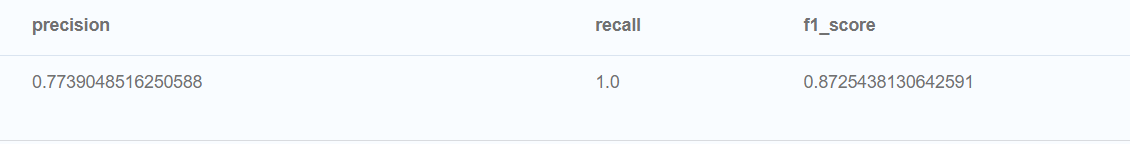
\includegraphics[width=\linewidth]{NC_precision_recall_f1score.png} % Replace with your image file
    \caption{Precision Recall and F1 Score}
    \label{fig:NC_Precision_Recall}
\end{figure}

The high recall value indicates that the classifier successfully predicted nearly all actual instances of each domain class. However, the slightly lower precision suggests that there were some false positives, indicating the need for improved feature representation or model tuning.

\subsubsection{Iteration 2 -- Embedding = 128, Number of Trees = 25}

\begin{itemize}
  \item \textbf{Test Accuracy:} 0.59
  \item \textbf{Test F1 Score:} 0.53
  \item \textbf{Out-of-Bag (OOB) Error:} 0.49
\end{itemize}

\begin{figure}[h]
  \centering
  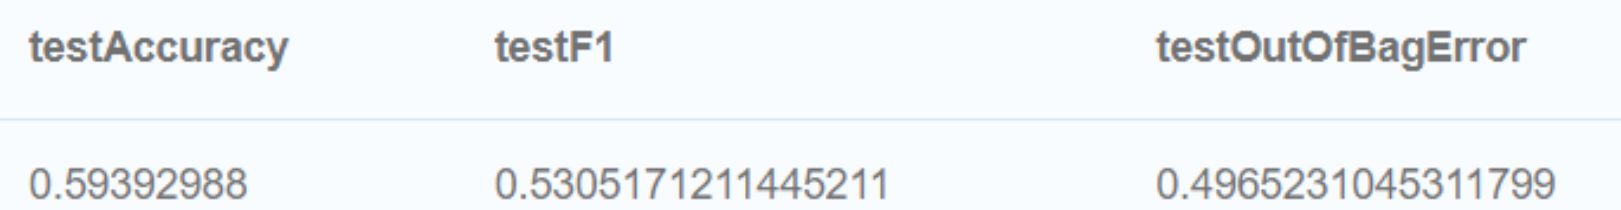
\includegraphics[width=\linewidth]{NC_model_training_output_2.png} 
  \caption{Output after training pipeline with embedding = 128 and trees = 25}
  \label{fig:classification_metrics_2}
\end{figure}

\begin{itemize}
  \item \textbf{Accuracy:} 0.78
  \item \textbf{Precision:} 0.78
  \item \textbf{Recall:} 1.00
  \item \textbf{F1 Score:} 0.88
\end{itemize}

\begin{figure}[H]
    \centering
    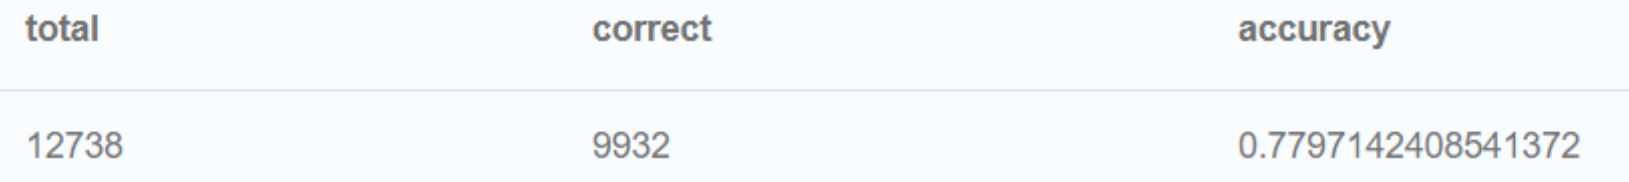
\includegraphics[width=\linewidth]{NC_accuracy_2.png} % Replace with your image file
    \caption{Accuracy for embedding = 128 and trees = 25}
    \label{fig:accuracy_2}
\end{figure}

\begin{figure}[H]
    \centering
    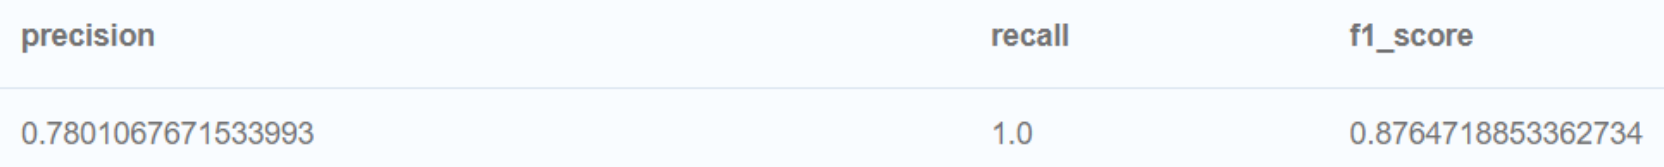
\includegraphics[width=\linewidth]{NC_precision_recall_f1score_2.png} % Replace with your image file
    \caption{Precision Recall and F1 Score for embedding = 128 and trees = 25}
    \label{fig:NC_Precision_Recall_2}
\end{figure}

The change in embedding does not show any significant change in the model output.\\

\subsubsection{Iteration 3 -- Embedding = 64, Number of Trees = 40}

\begin{itemize}
  \item \textbf{Test Accuracy:} 0.63
  \item \textbf{Test F1 Score:} 0.56
  \item \textbf{Out-of-Bag (OOB) Error:} 0.44
\end{itemize}

\begin{figure}[h]
  \centering
  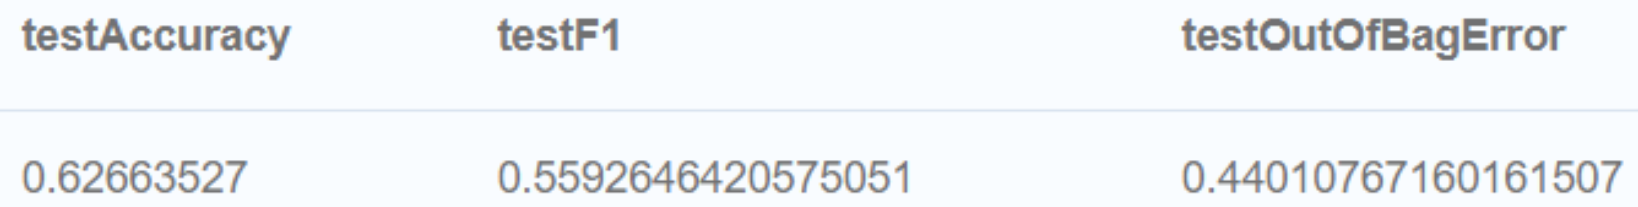
\includegraphics[width=\linewidth]{NC_model_training_output_3.png} 
  \caption{Output after training pipeline with embedding = 64 and trees = 40}
  \label{fig:classification_metrics_3}
\end{figure}

\begin{itemize}
  \item \textbf{Accuracy:} 0.79
  \item \textbf{Precision:} 0.80
  \item \textbf{Recall:} 1.00
  \item \textbf{F1 Score:} 0.88
\end{itemize}

\begin{figure}[h]
    \centering
    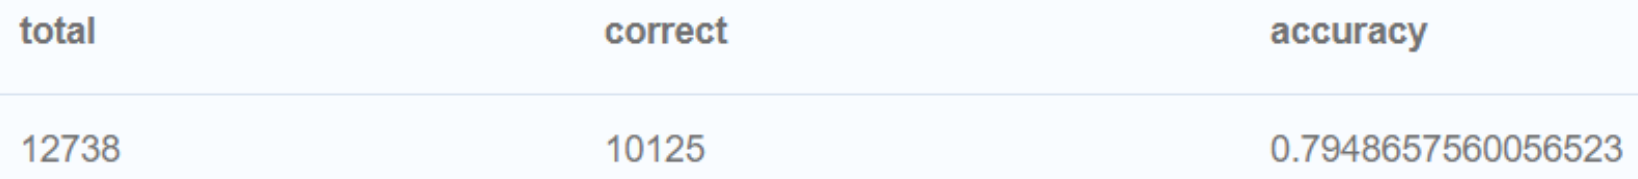
\includegraphics[width=\linewidth]{NC_accuracy_3.png} % Replace with your image file
    \caption{Accuracy for embedding = 64 and trees = 40}
    \label{fig:accuracy_3}
\end{figure}

\begin{figure}[h]
    \centering
    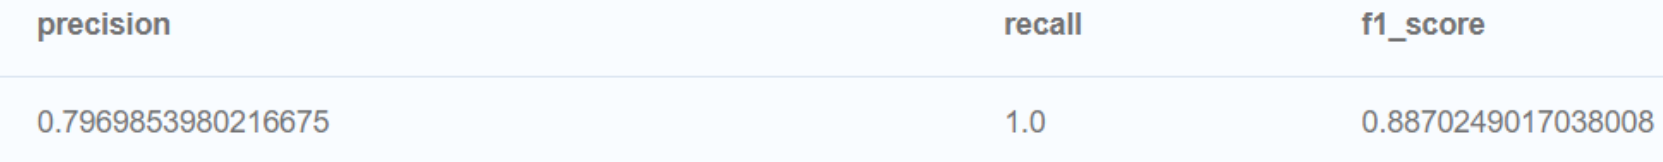
\includegraphics[width=\linewidth]{NC_precision_recall_f1score_3.png} 
    \caption{Precision Recall and F1 Score for embedding = 64 and trees = 40}
    \label{fig:NC_Precision_Recall_3}
\end{figure}

The increase in the number of trees for the random forest model slows a slight betterment in the results of 
accuracy and precision.


\subsection{Link Prediction Results}
The link prediction task evaluated three approaches to predict future author collaborations: a heuristic method and two machine learning iterations using FastRP and Node2Vec embeddings. We also tried using Fastrp instead of logistic regression for training, the code for which is avaliable on the repository under \texttt{LinkPredictionUsingRandomForest.pdf}  but discarded it midway due to the model taking taking too much time to train. Each iteration built upon the previous, addressing limitations and improving predictive performance.

\subsubsection{Heuristic Approach}
The heuristic approach employed a rule-based method to identify potential collaborations by computing a similarity score for author pairs without prior co-authorship. The methodology involved:

\begin{itemize}
    \item \textbf{Identifying Influential Authors}: The PageRank algorithm was used to select authors with a score greater than 0.1, indicating high influence in the co-authorship network.
    \item \textbf{Selecting Potential Collaborators}: For each influential author, we considered authors who shared the same research domain (\texttt{domain\_id}), had not previously collaborated, and had published more than two papers.
    \item \textbf{Calculating Similarity Scores}: A score was computed as:
    \begin{itemize}
        \item 0.3 $\times$ (normalized paper count of author 1 $\times$ normalized paper count of author 2).
        \item 0.3 $\times$ (normalized citation count of author 1 $\times$ normalized citation count of author 2).
        \item 0.4 if the authors shared the same research domain.
    \end{itemize}
    \item \textbf{Incorporating Citation Relationships}: Added 0.2 if one author’s papers cited the other’s, and an additional 0.2 for reciprocal citations.
    \item \textbf{Filtering and Ranking}: Pairs with a final score above 0.5 were ranked by score to identify likely collaborations.
\end{itemize}

This approach leveraged domain knowledge and network structure to provide an interpretable baseline without machine learning. The top predicted collaborations are shown in Figure \ref{fig:link_prediction_heuristic}.

\begin{figure}[h]
    \centering
    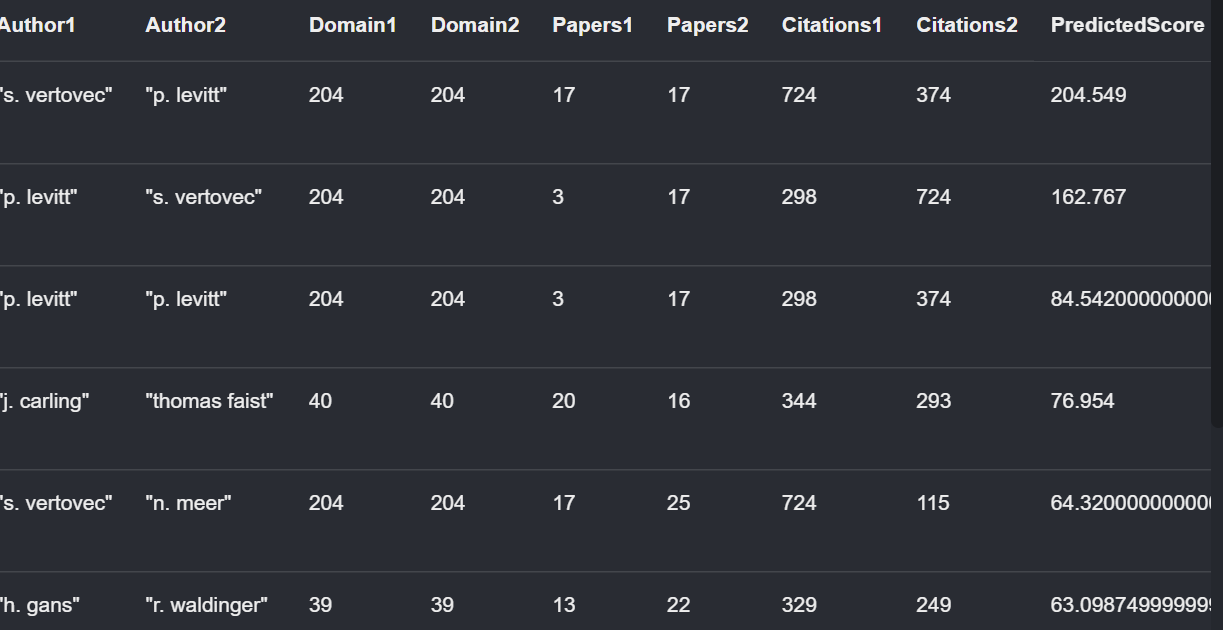
\includegraphics[width=\linewidth]{heuristic_results.png}
    \caption{Top Predicted Collaborations from Heuristic Approach}
    \label{fig:link_prediction_heuristic}
\end{figure}

As a non-ML method, standard metrics like AUPRC were not computed. The effectiveness was assessed qualitatively through the predicted pairs and their scores, higher predicted scores showed more likely possible future collaborations.

\subsubsection{Iteration 1 -- FastRP Embeddings}
The first machine learning iteration introduced Fast Random Projection (FastRP), with features extracted via the Hadamard product and fed into a logistic regression model. The model was trained with an 80/20 train-test split and negative sampling (ratio 1.0). Unlike the heuristic approach, this iteration used a classical ML pipeline, enabling quantitative evaluation.

The performance metrics were:
\begin{itemize}
    \item \textbf{AUPRC (Test)}: 0.73
    \item \textbf{Validation AUPRC (avg)}: 0.72
    \item \textbf{Outer Train AUPRC (avg)}: 0.72
\end{itemize}

\begin{figure}[h]
    \centering
    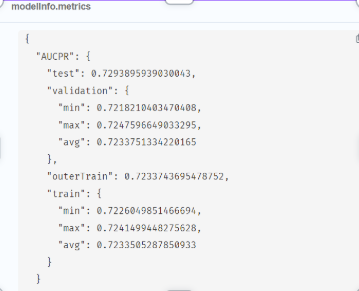
\includegraphics[width=\linewidth]{fastrp_metrics_1.png}
    \caption{Model Metrics for FastRP Iteration}
    \label{fig:link_prediction_fastRP_metrics}
\end{figure}

Compared to the heuristic approach, this iteration offered scalability and learned representations, achieving a test AUPRC of 0.727. However, the predicted probabilities clustered around 0.5 (Figure \ref{fig:link_prediction_fastRP_probabilities}), indicating limited confidence in distinguishing likely from unlikely collaborations. This clustering suggested that FastRP embeddings might not fully capture the nuanced relationships needed for effective link prediction.

\begin{figure}[h]
    \centering
    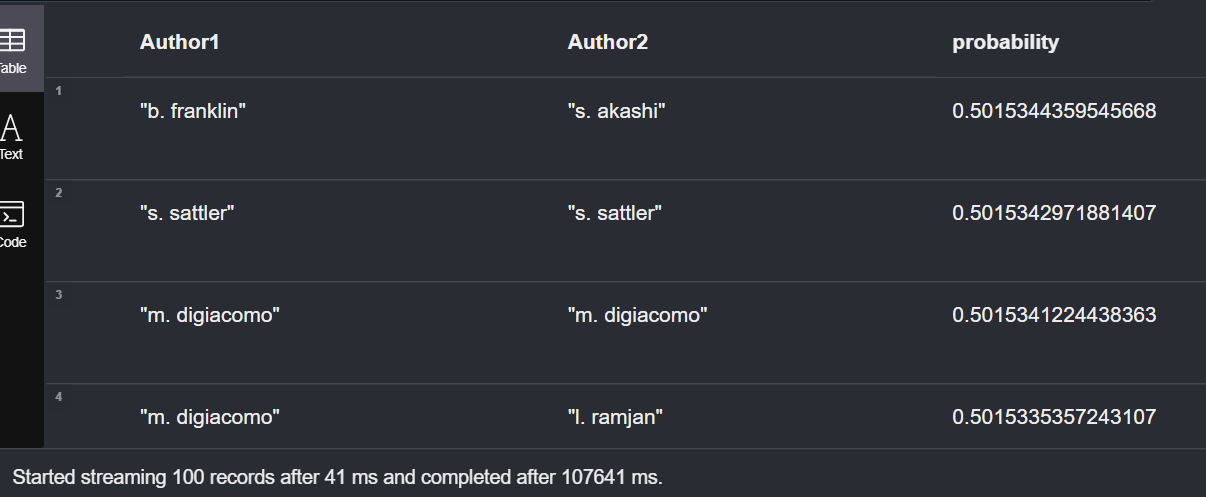
\includegraphics[width=\linewidth]{fastrp_results_1.png}
    \caption{Results for FastRP Iteration}
    \label{fig:link_prediction_fastRP_probabilities}
\end{figure}

The shift to an ML pipeline was a significant improvement over the heuristic method’s manual scoring, but the probability clustering highlighted a need for better embedding techniques.

\subsubsection{Iteration 2 -- Node2Vec Embeddings}
To address the probability clustering issue, the second iteration employed Node2Vec embeddings (64 dimensions, walk length 80, 10 walks per node), the pipeline remained similar, using Hadamard product feature extraction and logistic regression, with the same 80/20 train-test split and negative sampling. Additionally, this iteration corrected an error from earlier iterations by ensuring unique author pairs (author1.id < author2.id) to avoid self-loops.

The performance metrics were:
\begin{itemize}
    \item \textbf{AUPRC (Test)}: 0.677
    \item \textbf{Validation AUPRC (min)}: 0.668
    \item \textbf{Validation AUPRC (max)}: 0.676
    \item \textbf{Validation AUPRC (avg)}: 0.671
    \item \textbf{Outer Train AUPRC (min)}: 0.670
    \item \textbf{Outer Train AUPRC (max)}: 0.673
    \item \textbf{Outer Train AUPRC (avg)}: 0.671
\end{itemize}

\begin{figure}[h]
    \centering
    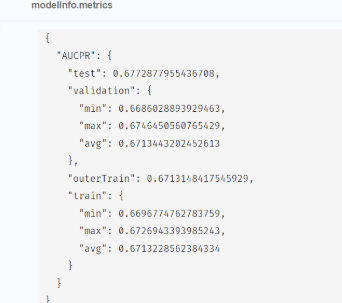
\includegraphics[width=\linewidth]{node2vec_metrics_2.png}
    \caption{Model Metrics for Node2Vec Iteration}
    \label{fig:link_prediction_node2vec_metrics}
\end{figure}

Compared to the FastRP iteration, Node2Vec resulted in a lower test AUPRC (0.677 vs. 0.729) but significantly improved the probability distribution, showing greater variation with probabilities ranging from 0.9536 to 0.9738 (Figure \ref{fig:link_prediction_node2vec_probabilities}). They showed much more variation when top 10 was changed to top 1000 while displaying the probabilities. This wider range indicated better calibration, enabling the model to confidently distinguish between likely and unlikely collaborations. The improvement stemmed from Node2Vec’s ability to balance local and global graph structures through biased random walks, making it more suitable for practical applications despite the lower AUPRC. The correction of self-loops further enhanced the model’s reliability.

\begin{figure}[h]
    \centering
    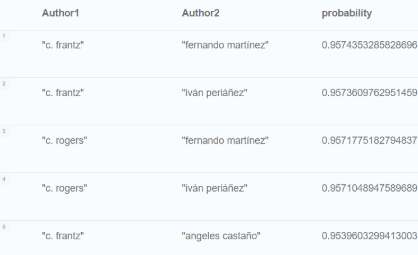
\includegraphics[width=\linewidth]{node2vec_results_2.png}
    \caption{Results for Node2Vec Iteration}
    \label{fig:link_prediction_node2vec_probabilities}
\end{figure}

The Node2Vec model was selected as the final model due to its superior probability calibration, offering a robust solution for predicting future collaborations.
\section{Discussion}
The node classification task demonstrated that structural features like Louvain community IDs and FastRP embeddings can effectively predict an author's research domain, with the third iteration (64-dimensional embeddings, 40 trees) achieving the best performance (Accuracy: 0.79, F1 Score: 0.88). However, limitations included low-informative embeddings for authors with few connections and ambiguity from interdisciplinary authors, leading to some misclassifications.

For link prediction, the node2vec-based model was preferred over fastRP due to its varied probability estimates, despite a slightly lower AUPRC. The fastRP model's probabilities clustered around 0.5, suggesting limited discriminative power. Early iterations incorrectly included self-loops, which was corrected in the final model by ensuring unique author pairs.

\subsection{Limitations and Challenges}
A key limitation was the quality of node embeddings. Several authors—particularly those with few or no co-authors—received zero or low-informative embedding vectors, which hindered classification accuracy. Additionally, the presence of interdisciplinary authors, who collaborate across multiple research domains, introduced ambiguity in both graph structure and labels. These factors contributed to misclassifications and highlight the need for more robust features beyond network structure.
Also, the training of the model was a resource heavy task, forcing us to limit our iterations for this task to only 3. Predictions also took really long to generate and we encountered lots of memory errors. Link prediction faced challenges with embedding quality and the need for more diverse features. The heuristic approach in the first iteration, while insightful, was not integrated into the ML pipeline, limiting its impact.

\subsection{Alternative Approaches}
For node classification, Node2Vec or Graph Neural Networks (GNNs) could capture more nuanced structures. Additionally, incorporating non-structural node features—such as publication keywords, journal categories, or citation counts—could enrich the feature set and provide context where structural signals are weak. These features could be extracted using NLP techniques applied to paper titles or abstracts.For link prediction, combining heuristic scores (e.g., from the first iteration) with learned embeddings or using GNNs could improve accuracy, clustering coeffecient can be incorporated as well.

\subsection{Possible Extensions}
Semi-supervised learning could infer domain labels for unlabeled authors. For link prediction, temporal features (e.g., collaboration recency) or additional metrics (e.g., common neighbors) could be explored. Hybrid models integrating multiple embedding techniques may further enhance both tasks.

\bibliographystyle{IEEEtran}
\bibliography{references.bib}

\end{document}
